\chapter{Deformation studies of a ladder under the test beam}

  The first full-scale prototype which embeds twelve sensors glued on a copper flex-cable and a 8 \% density \gls{SiC} foam was tested in November 2011 at CERN-SPS facility with a pions beam of 120 GeV.
  The motivations to perform such a test in real conditions are to, firstly, make sure that the ladder is working properly, secondly, that the sensors have a homogeneous response, and to point the benefits of a double sided measurement.
  This chapter does not aim to present the test beam campaign and all the results, but to focus on a specific study of the ladder's deformation.
  The reader can get some of the results here\todo{REF: loic's thesis}.
  This chapter will present the test beam facility, as well as the experimental set-up.
  Then, it will discuss a method to estimate the deformation of a ladder and how to overcome the deviations obtained during the analysis. 
  Finally, the benefits of double-sided measurements will be introduced.
  
  \minitoc

  \section{PLUME-V1 tested at CERN-SPS}

    \subsection{Test beam facility}

    The test beam was performed at CERN-SPS in the North hall on the H6 beam line.
    The spill structure is 9.6 s with a dead time of 45.6 s. 
    The test bean set-up is composed of 4 standards 120 $\mu\text{m}$ thinned Mi26 used as telescope and the DUT. 
    The reference planes are at 8 sigma S/N cut and stabilized to a temperature of 15 degrees Celsius.
    Most of the runs are taken with a trigger frequency between 2 and 8 kHz except for two days on which it was between 1 and 1.3 kHz on a scintillator of $7 \times 7 \text{mm}^2$.
    
    \subsection{Experimental set-up}

      \subsubsection{Reference plane and coordinate system}

    During the test beam, a telescope made of four reference planes mounted on two arms was used.
    The reference planes are MIMOSA-26 sensors thinned down to 120 $\mu\text{m}$.


     \begin{itemize}
       \item Beam structure
       \item Telescopes
     \end{itemize}

    \begin{figure}
      %\centering
      \missingfigure{TB geometries}
    \end{figure}

    The origin of the global coordinate system is determined with respect to the center of the two reference planes arms.
    The Z axis is going along the beam direction, the x axis corresponds to the horizontal direction and the y axis to the vertical direction.
    The local coordinate system is chosen at the center of a sensor, with w perpendicular to the plane, u is defined along the row and v along the columns.
    The figure~\ref{fig:labCoordinates} summarises the global and local coordinate system.

    \begin{figure}
      \centering
      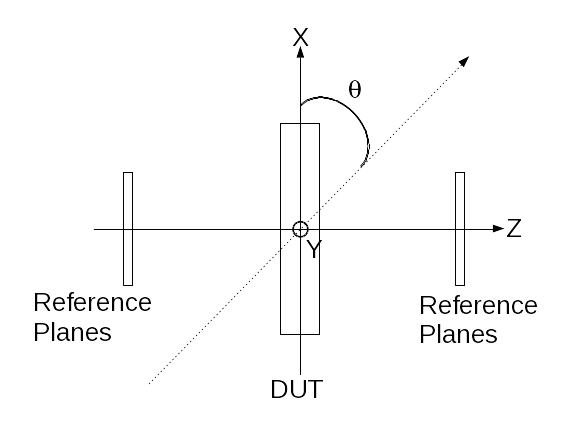
\includegraphics[width = 0.7\textwidth]{Pictures/deformation/lab_frame.png}
      \caption{Drawing of the laboratory coordinates.}
      \label{fig:labCoordinates}
    \end{figure}

      \subsubsection{Data Acquisition}

      The acquisition system is limited to eight sensors. 
      Four inputs are necessary for the telescope, thus only four sensors on the PLUME ladder can be connected, two on each side of the mechanical structure.
      Nevertheless, as the scintillator has a detection area of $7\times 7\text{mm}^2$, it is not mandatory to record the other sensors.

    \subsection{Software analysis}


      TAF:
      \begin{itemize}
        \item ROOT/C++
      \end{itemize}

  \section{Spatial resolution studies}
   
    One of the measurement performed during the analysis is to determine the pointing resolution of the ladder.
    The sensors used are well-known and they should have a pointing resolution similar to the one expected, regardless the mechanical structure.
    Any deviations might point out an impact of the mechanical structure on the whole system.
    To get the better understanding, different running conditions were performed: different air flow speed to cool the ladder, different threshold levels and different orientation on of the ladder with respect to the beam.

    \subsection{Normal incidence track}


    \subsection{Ladder tilted in one direction}
    
    This test-beam results have already been discussed (reference to paper and thesis) and results, such as the efficiency or ... are no going to be presented.

    \begin{figure}
      %\centering
      \missingfigure{Track-hit residual as a function of the hit position (normal incidence)}
    \end{figure}

    \begin{figure}
      %\centering
      \missingfigure{Track-hit residual as a function of the hit position (tilt)}
    \end{figure}

    \begin{figure}
      %\centering
      \missingfigure{Residual (tilt and normal incidence)}
    \end{figure}

    \begin{figure}
      %\centering
      \missingfigure{Explanation of deviations}
    \end{figure}
    
  \section{Benefits of double-sided measurement}

  %\todo{REF Loic thesis for TB@CERN results}
